\documentclass[10pt]{article}
\usepackage[utf8]{inputenc}
\usepackage{parskip}
\usepackage[a4paper, margin=1.5in]{geometry}
\usepackage{graphicx}
\usepackage{hyperref}
\usepackage{listings}
\usepackage{array}

\renewcommand{\arraystretch}{1.5}

\title{Task 1 Report}
\date{11/11/2019}
\author{Federico Fregosi, Mirko Laruina,\\
        Riccardo Mancini, Gianmarco Petrelli}

\begin{document}
\pagenumbering{gobble}
\maketitle
\vfill
% \setcounter{tocdepth}{1}
\tableofcontents
\vfill
\clearpage
\setcounter{page}{1}
\pagenumbering{arabic}

\section{Application Specifications}
\subsection{Application overview}
The application is a messaging system where registered users can create an 
account, exchange text messages and make groups.

A registered user can initiate a chat with another user, create a new group chat
(of which he becomes the admin) and send messages to the chats he belongs to,
as well as receiving messages from those chats. He can also leave a group.

A group admin can add and remove new users to the group. He cannot assign his
powers to another user in the group and if he leaves the group, the latter 
is deleted.

Everytime a user views a chat, all the latest messages from the chat are fetched from 
the server and shown to the user.

\subsection{Actors}
Anonymous user, registered user, group admin and a time-based event.

\subsection{Requirement Analysis}
\subsubsection{Functional requirements}

An \textbf{anonymous user} must be able to register in order to become a 
\emph{registered user}.

A \textbf{registered user} must be able to:
\begin{itemize}
    \item Send a message to a chat
    \item Read chat messages
    \item Create a private chat
    \item Create a group chat
\end{itemize}

A \textbf{group admin} must be able to:
\begin{itemize}
    \item Add users to the group
    \item Remove users from the group
\end{itemize}

The \textbf{time-based event} updates the user interface on regular intervals
to show new received messages from the current chat, if any.

\subsubsection{Non-Functional requirements}
TODO

\clearpage
\section{Design}
\subsection{Use-case diagram}
\begin{figure}[h!]
    \centering
    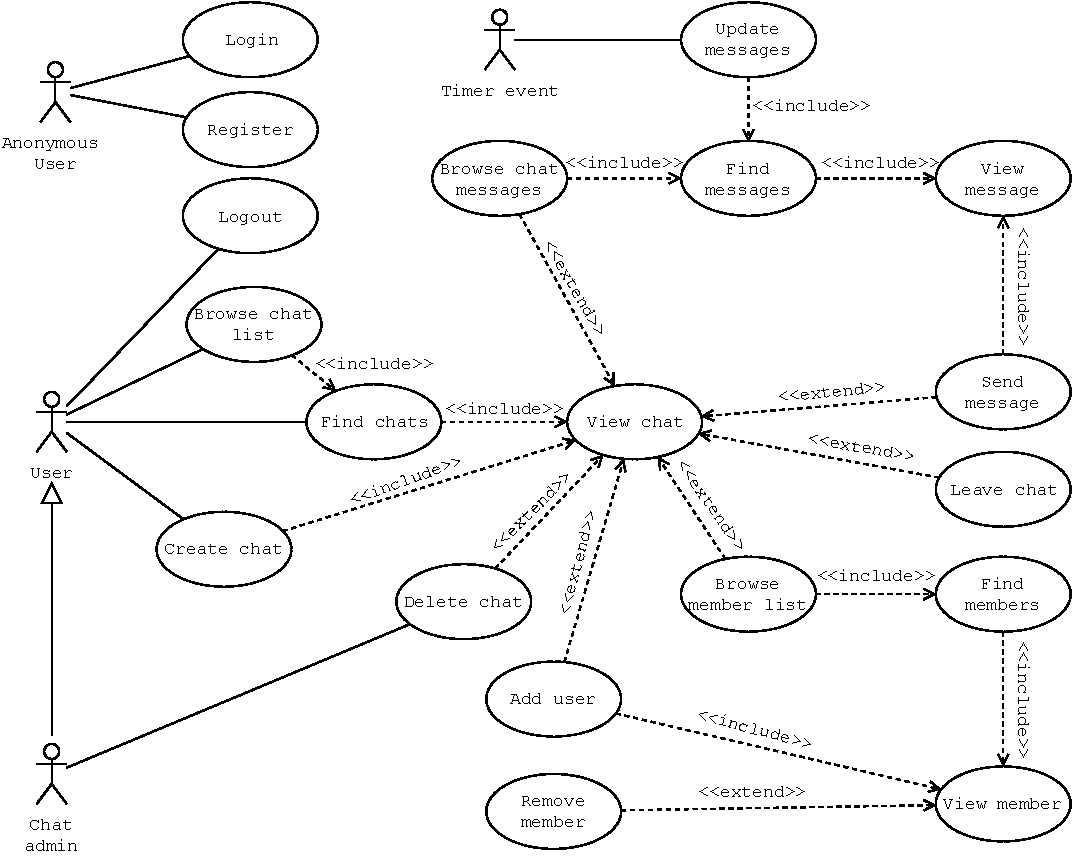
\includegraphics[width=\textwidth]{figs/use_case_diagram}
    \caption{Use-case diagram. Use-cases indicated with a star (\texttt{*})
        require the user to be the chat administrator.}
    \label{fig:usecase}
\end{figure}

\subsection{Class diagram}
\begin{figure}[h!]
    \centering
    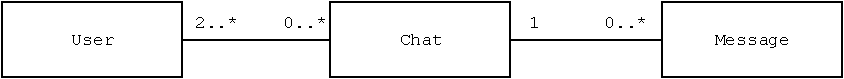
\includegraphics[width=\textwidth]{figs/class_diagram}
    \caption{Class diagram for the identified entities.}
    \label{fig:class_diagram}
\end{figure}

Figure~\ref{fig:class_diagram} shows the class diagram derived from the specifications. 
It can be seen that we chose to keep it as simple as possible by not making  
any distinction between \emph{private chats} and \emph{group chats}, 
creating a single \emph{Chat} entity.

\subsection{Software Architecture}
TODO

The proposed software architecture is a classic three-layer architecture:
\begin{enumerate}
    \item database (MySQL)
    \item server back-end (Java + Spring)
    \item user web app (ReactJS)
\end{enumerate}

\clearpage
\section{Implementation}

\subsection{Database}
\subsubsection{Relational DB Design}
\begin{figure}[]
    \centering
    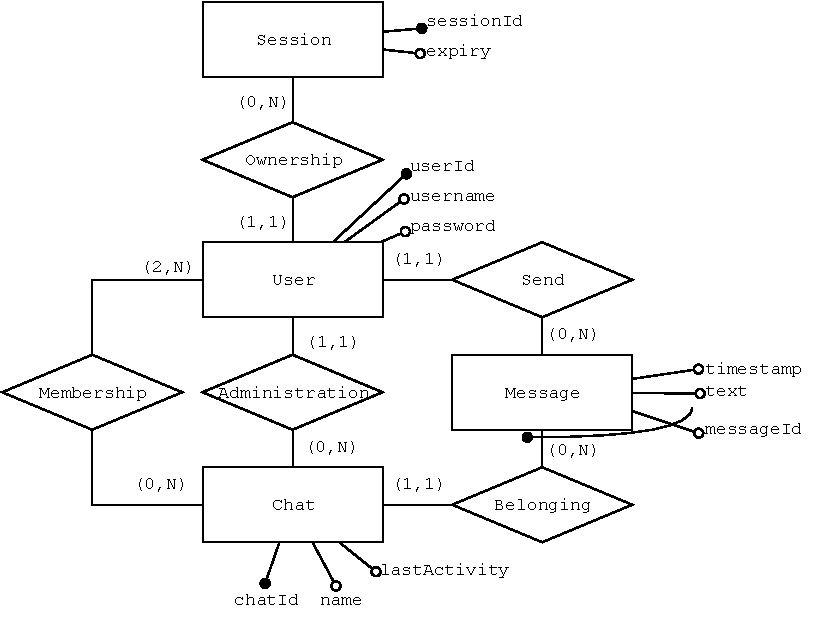
\includegraphics[width=\textwidth]{figs/ER}
    \caption{ER diagram for the database.}
    \label{fig:er}
\end{figure}

Figure~\ref{fig:er} shows the ER diagram of the MySQL database. Every \emph{User} 
is identified a \emph{userId} and has got a unique \emph{username} and a 
\emph{password}. The user can be a member of many \emph{Chats} and can 
be the administrator of many \emph{Chats}. On the other hand, a \emph{Chat} 
can be administered by only one \emph{User}. A \emph{User} can send a 
\emph{Message} to a \emph{Chat}. Each \emph{User} and each \emph{Chat} can 
have many \emph{Messages} while a \emph{Message} can belong to one \emph{Chat}
and one \emph{User} only. The \emph{Session} represents a logged user session.
Each \emph{User} can have many open \emph{Sessions}.

Once the database had been created, we filled it with random test data using the free
service available at \url{http://filldb.info/}. Generated data is not perfect, 
since some more complex functional constraints could not be included in the 
generation. However, that was sufficient for the first functional tests of the
application.

\subsubsection{JPA}
Given the database, the Java implementation using JPA was very fast, especially
compared to using plain SQL. We made use of both one-to-many and many-to-many 
relationships as it can be seen from the ER diagram.

TODO

\subsection{Java backend}
The Java backend provides simple REST APIs for managing the chat application. 
In order to do so, it uses the \emph{Spring} framework\footnote{More information
at \url{https://spring.io/}}.
The list of the APIs and their description can be found in the 
\texttt{docs/api.md} file. The APIs return a JSON document, generated using
\emph{Google GSON}\footnote{More information at 
\url{https://github.com/google/gson}}, which is interpreted and shown to the user
by the ReactJS frontend.
These APIs are implemented using a simple database abstraction layer which provides 
corresponding APIs to the database. This is implemented in Java 
using a generic \emph{DatabaseAdapter} interface that can be implemented to 
provide access to different databases (as we have done in this Task with plain SQL, 
JPA and levelDB implementations). The database backend can be set from a configuration
file, where some other db-specific settings can be set.

\subsection{ReactJS frontend}
The fronted has been developed using the \emph{ReactJS} framework\footnote{More
information at \url{https://reactjs.org/}}. An overview of the main functions 
is available in the user guide (\texttt{docs/user\_guide/user\_guide.pdf}).

Regarding the implementation, the most notable thing is the timer-based event
that updates the UI. In particular, the client makes a request to the server
every second for updating the list of chats and every half second for updating 
the list of messages in the current chat.

\subsection{Limitations}
\paragraph{Passwords}
For the sake of simplicity, password hashing has not been implemented into the 
application. However, this could be simply integrated with a future update.

\paragraph{Polling}
In the current implementation, the server is polled every second for updating 
the list of chats and every half second for updating the list of messages. This 
is indeed a great load on the server in case there are many clients connected 
at the same moment. 
This problem has been alleviated by requesting only a subset of the chat 
messages, based on the timestamp on the latest received message.
However, 
a more appropriate way to handle it would be having a kind of notification API
that can be ``long polled''\footnote{A ``long poll'' is when the client 
makes a request to the server and the server does not respond until new 
information is available, at the cost of timing out the connection, at which 
point a new request is made.} by the client.

\section{Testing and Evaluation}

The database APIs have been tested using some test units through \emph{JUnit4}
\footnote{More information at \url{https://junit.org/junit4/}} before being 
integrated with the ReactJS frontend.

TODO

\end{document}
